\documentclass[11pt]{article}

\usepackage[margin=1in]{geometry}
\usepackage[dvipsnames]{xcolor}
\usepackage{graphicx}
\usepackage{booktabs}
\usepackage[hyphens]{url}
\usepackage{hyperref}

\hypersetup{
  colorlinks=true,
  linkcolor=blue!60!black,
  citecolor=blue!60!black,
  urlcolor=blue!60!black,
  breaklinks=true,
  pdftitle={Quantifying Arroyo's Asthenocoria Sign},
  pdfauthor={Walker Kirkpatrick}
}

\title{Quantifying Arroyo's Asthenocoria Sign: \\
A Low-Cost Embedded Pupillography System \\
for Naturopathic Clinical Screening}
\author{Walker Kirkpatrick, ND}
\date{September 2026}

\begin{document}
\maketitle

\begin{abstract}
Arroyo's asthenocoria sign, first described in 1924, is the failure of the pupil
to sustain constriction under continuous light exposure---a phenomenon
historically associated with adrenal insufficiency in naturopathic and
functional medicine. Despite nearly a century of clinical use, the test has
remained a subjective bedside observation dependent on examiner skill and
patient cooperation. We present \texttt{arroyo-pi}, an open-source embedded
pupillography system that quantifies the Arroyo sign using a 940\,nm
near-infrared LED, a NoIR camera module (Arducam IMX462 for Raspberry Pi or
IMX219-NoIR for Jetson Orin Nano), and a Python analysis core built on OpenCV
dark-pupil detection. The system records pupil diameter via the
pupil-to-iris ratio (PIR) method, calibrated against a horizontal visible iris
diameter of 11.7\,mm, and applies a deterministic analysis pipeline: baseline
median estimation, maximum constriction search, escape detection at 15\% of
constriction amplitude sustained for 2\,s, oscillation counting with
running-median detrending, and four-band grading (healthy $\geq$\,20\,s, mild
10--20\,s, fatigue 5--10\,s, exhaustion $<$\,5\,s). A suite of 25 unit tests
with synthetic pupillograms validates all grading bands, edge cases, and
symmetry comparisons. The system is the hardware successor to an Apple Vision
Pro prototype, replacing proprietary camera restrictions with a sub-\$100
embedded platform. We frame the tool honestly: it measures pupillary behavior,
not adrenal function, and the grading thresholds are functional-medicine
screening bands, not clinically validated diagnostic criteria. The system
enables objective trend tracking and removes observer bias from a test that
has lacked instrumentation for a century.
\end{abstract}

\section{Introduction}

The pupillary light reflex is among the most accessible windows into autonomic
nervous system function. A clinician can observe it with nothing more than a
penlight and a darkened room. Yet this accessibility has paradoxically
constrained its clinical utility: without instrumentation, the observation
remains qualitative, subject to inter-examiner variability, and impossible to
track longitudinally with any rigor.

Arroyo's asthenocoria sign---the failure of the pupil to hold constriction
under sustained light---exemplifies this gap. Described in 1924 by Carlos~F.\
Arroyo as a correlate of adrenal insufficiency, the sign has persisted in
naturopathic and functional medicine practice for a century without ever
transitioning from subjective observation to objective measurement. A
practitioner shines a light across the patient's eye, watches the pupil
constrict, and then waits to see whether constriction is maintained or the
pupil redilates despite continued illumination. The result is a judgment call,
graded by a stopwatch at best and by impression at worst.

This paper presents \texttt{arroyo-pi}, a low-cost embedded pupillography
system that replaces the subjective exam with instrumented measurement. The
system uses near-infrared illumination invisible to the human eye, a
consumer-grade NoIR camera, and an OpenCV-based tracking pipeline to record
pupil diameter continuously throughout the test. A Python analysis core then
applies deterministic algorithms to detect pupillary escape, quantify hold
time, and assign a grade. The hardware platform is a Raspberry Pi~4/5 or
NVIDIA Jetson Orin Nano, making the system accessible to clinics that cannot
justify research-grade pupillometry equipment.

We position this system as a screening and trend-tracking instrument, not a
diagnostic device. The physiological relationship between sustained pupillary
behavior and adrenal function is not established by conventional
endocrinology, and the grading thresholds used in functional medicine
practice have not been clinically validated. What the system provides is
objectivity, repeatability, and freedom from observer bias---enabling
practitioners to track changes over time with quantitative confidence.

\section{Historical Background}

Carlos~F.\ Arroyo (1892--1928) was a physician whose 1924 publication in the
\textit{Medical Journal and Record} (January~2, 1924) described a pupillary
sign he observed in patients with adrenal insufficiency. Arroyo termed this
sign \textit{asthenocoria}---from the Greek \textit{astheneia} (weakness) and
\textit{kore} (pupil)---characterizing it as a sluggishness or weakness of the
pupillary light reflex under sustained illumination~[3,4].

The Farlex Medical Dictionary defines asthenocoria as ``sluggishness of the
pupillary light reflex,'' attributing the eponym \textit{Arroyo sign} to the
same phenomenon~[3]. The IQB Spanish Medical Dictionary similarly records the
\textit{Signo de ARROYO} as a sluggish pupillary reaction to light~[4].

Arroyo's original description, as preserved in the Thyroid Patient Advocacy UK
source~[1], reads:

\begin{quote}
\small\itshape
When exploring the pupil area reflex, I found that in the iris of those cases
(adrenal insufficiency), although reacting readily to light, the contraction
(of the iris) was flabby, lazy, in a word asthenia. By making the patient look
at the light we see that immediately after the initial mitosis the pupil
starts to dilate slowly as if it does not want to, seems to try to contract
again but the dilation gains the upper hand and, after a fight between miosis
and mydriasis lasting for about 40 seconds, the pupil remains dilated in spite
of the persistence of the exciting agent (the light). This sign is consistent
and present in all cases of hypoadrenia in all of its clinical forms. In the
normal individual, it does not appear as I have investigated. All patients
presenting this sign, which I should like to call asthenocaria, have been
benefited by suprarenal medication.
\end{quote}

The protocol Arroyo described is straightforward: darken the room, shine a
light across one eye (not directly into it), and observe whether the initial
constriction is maintained or the pupil redilates despite continued
illumination. The sign is positive when redilation or oscillation occurs
under sustained light. Arroyo reported that the sign was absent in healthy
individuals and present in all clinical forms of hypoadrenia he
investigated~[1].

\section{Naturopathic and Functional Medicine Context}

Arroyo's test survived in naturopathic and functional medicine literature long
after it faded from conventional practice. The test is commonly known in
these traditions as the \textit{iris contraction test} or the \textit{pupil
response test}, and it appears in practitioner guides and patient-facing
resources as a self-administered screening tool for adrenal
dysfunction~[2,23,24,25].

James~L.\ Wilson coined the term ``adrenal fatigue'' in 1998 to describe a
putative syndrome of subclinical adrenal hypofunction characterized by
fatigue, salt craving, and impaired stress tolerance~[22]. Within this
framework, Arroyo's iris contraction test became a standard screening
instrument. Wilson's framework proposed that under chronic stress, the
adrenal glands progress through stages of alarm, resistance, and exhaustion,
and that pupillary instability reflects this progressive
decompensation~[22,30].

The grading thresholds most commonly cited in functional medicine literature
are~[2,23]:

\begin{itemize}
  \item \textbf{Healthy:} constriction held for 20 seconds or more
  \item \textbf{Mild disruption:} constriction held for 10--20 seconds
  \item \textbf{Fatigue:} constriction held for 5--10 seconds
  \item \textbf{Exhaustion:} constriction fails within 5 seconds
\end{itemize}

Some protocol variants specify the light source at 8 inches and 45 degrees
from the eye~[5], while others recommend a penlight held approximately 20\,cm
from the eye at a similar angle. The common elements are a dim room, a
sustained lateral light source, and timed observation of pupil behavior.

The test also appears in syntonic optometry, a branch of optometric practice
that uses light therapy. The \textit{Alpha Omega Pupil} concept in syntonic
optometry relates pupillary response to autonomic balance and visual field
constriction, drawing on similar observations of sustained constriction
capacity~[6].

We emphasize that these thresholds are \textbf{not} clinically validated.
They originate from clinical observation and practitioner tradition, not from
controlled studies with defined populations. The test functions as a
screening and trend instrument: a practitioner uses it to track changes
within an individual over time, not to diagnose a specific pathology. The
system described in this paper preserves these thresholds as configurable
parameters precisely because they represent the conventional practice the
system is designed to instrument.

\section{Physiological Basis}

\subsection{The Pupillary Light Reflex}

The pupillary light reflex (PLR) is the constriction of the pupil in response
to retinal illumination, mediated by a subcortical reflex arc. Light striking
the retina activates retinal ganglion cells whose axons travel via the optic
nerve to the pretectal nuclei in the midbrain. From there, signals reach the
Edinger--Westphal nuclei, whose parasympathetic fibers travel via the
oculomotor nerve to the sphincter pupillae muscle, producing
constriction~[7,8,27].

Pupil diameter is governed by the balance between parasympathetic
constriction (sphincter pupillae) and sympathetic dilation (dilator
pupillae). The parasympathetic pathway acts rapidly: light onset triggers
constriction within approximately 200--500\,ms. The sympathetic pathway acts
more slowly, modulating baseline pupil size and contributing to redilation
after light offset~[7].

\subsection{Pupillary Escape as a Normal Phenomenon}

Pupillary escape---the partial redilation of the pupil despite continued light
stimulation---is a \textbf{normal} physiological phenomenon, not inherently
pathological. Loewenfeld and her collaborators established that under
sustained illumination, the pupil initially constricts and then partially
redilates as the retinal response adapts~[26]. This escape reflects the
adaptation of the retinal photoreceptors and the dynamics of the neural
integpathway, not a failure of any specific organ system.

The degree of pupillary escape depends on stimulus intensity, adaptation
state, and individual variability. Under bright light, constriction is
well sustained; under dimmer or moderate light, escape is more
pronounced~[26,27]. This is a critical consideration for Arroyo's test:
the protocol uses a penlight at an angle, producing a moderate and somewhat
variable stimulus, which makes the amount of escape highly sensitive to
stimulus conditions.

\subsection{Melanopsin and Intrinsically Photosensitive Retinal Ganglion Cells}

A subset of retinal ganglion cells---intrinsically photosensitive retinal
ganglion cells (ipRGCs)---contain melanopsin, a photopigment with peak
sensitivity near 480\,nm. These cells contribute to sustained pupillary
constriction under continuous light, providing a tonic constriction signal
that complements the phasic response of rod and cone pathways~[26,27].

The melanopsin contribution helps explain why the pupil can maintain partial
constriction under prolonged illumination. However, the sustained-light
observation used in Arroyo's test differs fundamentally from flash
pupillometry: flash techniques measure the transient response to brief
stimuli, while Arroyo's protocol observes the sustained response over tens of
seconds, where adaptation, escape, and oscillation dynamics dominate.

\subsection{The Four Phases of the Pupillary Light Reflex}

The PLR under sustained light can be decomposed into four phases~[8,27]:

\begin{enumerate}
  \item \textbf{Latency:} The delay between light onset and the beginning of
        constriction, typically 200--500\,ms. The \texttt{arroyo-pi} system
        detects latency as the first frame where pupil diameter drops 5\%
        below baseline, sustained for 3 consecutive samples.
  \item \textbf{Constriction:} The active narrowing phase, reaching maximum
        constriction within 1--2\,s of light onset. The system searches for
        minimum pupil diameter within a 5\,s post-stimulus window.
  \item \textbf{Escape:} Partial redilation despite continued illumination,
        reflecting retinal adaptation and the balance of autonomic inputs.
        The system flags escape when the pupil redilates by 15\% or more of
        the constriction amplitude, sustained for at least 2\,s.
  \item \textbf{Recovery:} Return toward baseline after light offset, driven
        by sympathetic dilation and cessation of parasympathetic tone.
\end{enumerate}

\section{Clinical Limitations and Honest Framing}

We are deliberate about what this system does and does not measure.

``Adrenal fatigue'' is not a recognized diagnosis in conventional
endocrinology. The Endocrine Society and other major medical bodies do not
recognize it as a valid clinical entity, and the symptoms attributed to it
overlap substantially with other conditions~[29,31]. WebMD notes that
``adrenal fatigue'' as a concept lacks the scientific evidence required for
clinical acceptance~[29]. Medical News Today similarly reports that the term
is not supported by endocrinological research~[31].

The gold standard for diagnosing adrenal insufficiency is the ACTH
(cosyntropin) stimulation test, which measures cortisol response to exogenous
adrenocorticotropic hormone~[10]. This is a blood test performed in a
clinical laboratory, not a pupillary observation. Primary adrenal
insufficiency (Addison's disease) is rare and requires definitive
endocrinological workup~[10].

Asthenocoria itself is nonspecific. The Ulyclinic clinical reference notes
that Arroyo's sign can appear in various conditions and is not specific to
adrenal dysfunction~[9]. Pupillary escape is influenced by fatigue, lighting
conditions, medications, autonomic tone, age, and individual variability. A
positive Arroyo sign does not indicate adrenal pathology, and a negative sign
does not rule it out.

\textbf{The \texttt{arroyo-pi} system measures pupillary behavior---not
adrenal function.} It quantifies how long the pupil sustains constriction
under continuous light, how much it redilates, and whether it oscillates.
These are pupillary measurements. Any inference about adrenal status is a
clinical judgment made by the practitioner, not a measurement made by the
system.

The grading thresholds (20\,s, 10\,s, 5\,s) are functional-medicine screening
bands, not validated diagnostic criteria. They are useful for tracking trends
within an individual over time, which is how naturopathic practitioners
typically use the test~[24,25]. We preserve these thresholds in the system
as configurable parameters, and we explicitly label every report with a
reminder that the system is a screening instrument.

\section{System Architecture}

\subsection{Hardware}

The \texttt{arroyo-pi} system consists of three hardware components
(Figure~3):

\begin{itemize}
  \item \textbf{IR illumination:} A 940\,nm near-infrared LED provides
        illumination for the camera. The 940\,nm wavelength is invisible to
        the human eye and does not trigger the pupillary light reflex,
        allowing the camera to observe the pupil without itself altering
        pupil size~[18,19]. This is a critical design choice: visible
        illumination would confound the test by acting as an uncontrolled
        stimulus. The 940\,nm band is widely used in eye-tracking systems
        for this reason~[18,19].
  \item \textbf{Camera:} A NoIR (no infrared filter) camera module captures
        the eye under IR illumination. Two options are supported:
        \begin{itemize}
          \item \textbf{Raspberry Pi:} Arducam IMX462 Pivariety camera, a
                low-light-optimized sensor with a Starvis sensor suitable
                for IR imaging~[17].
          \item \textbf{Jetson Orin Nano:} IMX219-NoIR, the standard
                Raspberry Pi camera module V2 with the IR filter removed,
                connected via the Jetson's MIPI-CSI interface.
        \end{itemize}
        Both cameras operate at 30\,fps at 640$\times$480 resolution, which
        is sufficient for the temporal dynamics of the Arroyo test (pupillary
        changes occur over seconds, not milliseconds).
  \item \textbf{Compute:} Raspberry Pi~4 or 5, or NVIDIA Jetson Orin Nano.
        The Jetson provides GPU acceleration if needed for future
        deep-learning-based tracking, but the current OpenCV pipeline runs
        comfortably on CPU at 30\,fps.
\end{itemize}

The total hardware cost is under \$100, compared to thousands of dollars for
research-grade pupillometry equipment~[15,21].

\subsection{Software}

The software stack is implemented in Python with OpenCV for computer vision:

\begin{itemize}
  \item \textbf{Pupil tracking} (\texttt{tracker.py}): Dark-pupil detection
        under 940\,nm IR. The pipeline uses Haar cascade classifiers for
        face and eye region detection, Hough circle fitting for the iris
        boundary, and adaptive thresholding with contour analysis and
        ellipse fitting for the pupil. The pupil is identified as the darkest
        circular region within the eye ROI, scored by circularity, darkness,
        and size~[16].
  \item \textbf{PIR calibration:} The pupil-to-iris ratio (PIR) method
        converts pixel measurements to millimeters. The iris diameter serves
        as an internal calibration ruler, with the horizontal visible iris
        diameter (HVID) assumed to be 11.7\,mm (adult average). PIR is
        computed as pupil diameter divided by iris diameter, both in pixels,
        and multiplied by 11.7\,mm to obtain absolute pupil diameter. This
        approach avoids the need for external calibration and is robust to
        changes in camera distance~[27].
  \item \textbf{Analysis core} (\texttt{analysis.py}): A Python-native
        implementation of the Arroyo analysis algorithm, ported from the
        \texttt{arroyo-visionos} reference core. The algorithm detects
        pupillary escape, counts oscillations, and assigns a grade based on
        hold time. Section~\ref{sec:algorithm} describes the pipeline in
        detail.
  \item \textbf{CLI} (\texttt{main.py}): A command-line interface with three
        modes: \texttt{live} (camera exam), \texttt{demo} (synthetic data
        for testing without hardware), and \texttt{calibrate} (camera
        preview with tracking overlay for positioning).
\end{itemize}

\begin{figure}[htbp]
  \centering
  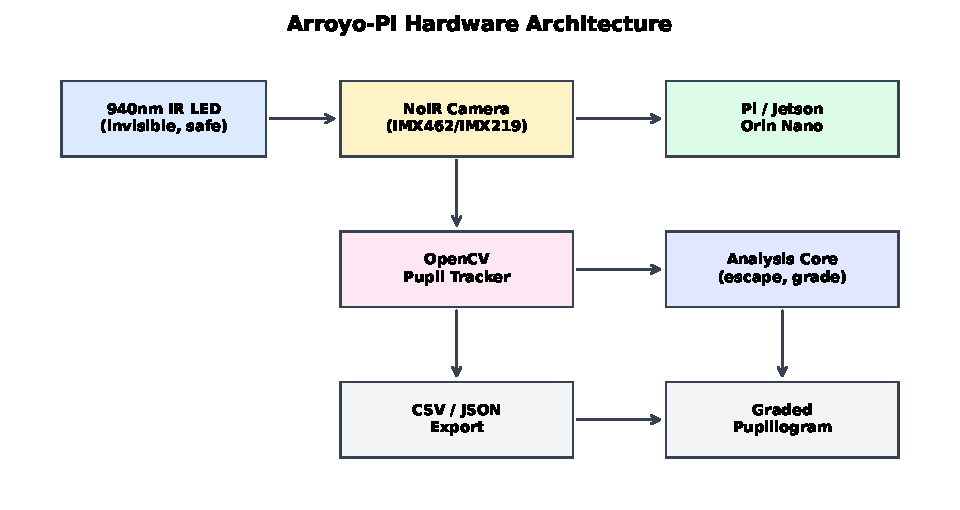
\includegraphics[width=0.90\textwidth]{figures/fig3_architecture.pdf}
  \caption{Hardware architecture block diagram. The 940\,nm IR LED provides
  invisible illumination; the NoIR camera captures the eye; the Raspberry Pi
  or Jetson processes frames in real time with OpenCV dark-pupil detection.}
\end{figure}

\section{Algorithm Details}
\label{sec:algorithm}

The analysis pipeline processes a time series of pupil measurements and
produces a graded result. Each step is implemented in \texttt{analysis.py}
and is deterministic---no machine learning or stochastic components are
involved. The algorithm operates on PIR (pupil-to-iris ratio) values rather
than raw pixel counts, providing scale invariance.

\subsection{PIR Interpolation of Invalid Frames}

The tracker marks frames as invalid when no pupil is detected (e.g., during
blinks or tracking loss). Invalid frames are linearly interpolated between
the nearest valid neighbors to produce a continuous PIR time series. If fewer
than 50\% of frames are valid, the recording is rejected as insufficient
data.

\subsection{Baseline Estimation}

The baseline PIR is computed as the median of all valid samples in the
2-second window preceding stimulus onset ($t_0$). If no pre-stimulus data is
available (e.g., the recording starts at or after stimulus onset), the first
2\,s of the recording are used and a quality warning is emitted. The median
is chosen over the mean for robustness against outliers and blink artifacts.

\subsection{Maximum Constriction Search}

The minimum PIR (maximum constriction) is found by searching the 5-second
window following stimulus onset ($t_0 \leq t \leq t_0 + 5$\,s). The
constriction amplitude is the difference between baseline PIR and minimum
PIR. If the amplitude is less than 5\% of baseline, the recording is graded
as ``no reflex''---no reliable constriction was detected.

\subsection{Escape Detection}

Escape is defined as redilation reaching 15\% of the constriction amplitude,
sustained for at least 2\,s. The algorithm scans the post-constriction time
series and, for each point where the relative redilation exceeds 15\%, checks
whether the redilation is maintained above 15\% for the subsequent 2\,s. The
first such sustained crossing defines the escape time. The hold time is the
interval from maximum constriction to escape onset. If no escape is detected,
the pupil is graded as ``held'' (constriction maintained for the full
recording).

\subsection{Oscillation Counting}

Oscillations---rhythmic fluctuations in pupil diameter after
constriction---are counted using a detrending and hysteresis approach:

\begin{enumerate}
  \item The post-constriction PIR series is detrended using a running median
        with a 3-second window, removing slow drift while preserving
        oscillations.
  \item A hysteresis band of $\pm$10\% of constriction amplitude is applied
        to the residual. The algorithm tracks direction state and counts
        zero-crossings of the hysteresis band, with each complete cycle
        (up-crossing followed by down-crossing) counted as one oscillation.
  \item The oscillation frequency is the cycle count divided by the
        post-constriction duration.
\end{enumerate}

Oscillations at 0.3\,Hz or above, combined with rapid escape, characterize
the exhaustion band.

\begin{figure}[htbp]
  \centering
  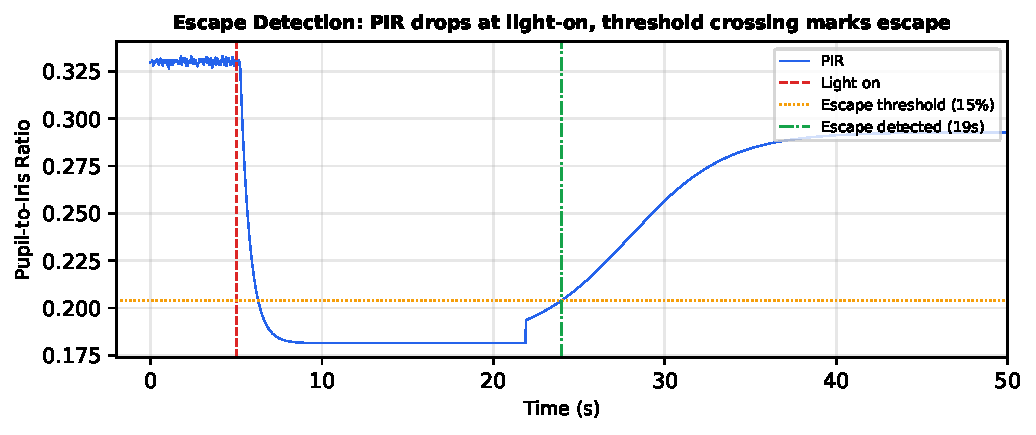
\includegraphics[width=0.95\textwidth]{figures/fig2_escape_detection.pdf}
  \caption{PIR time series showing the escape detection algorithm. The
  baseline median, maximum constriction, and 15\% escape threshold are
  annotated. The pupil redilates past the threshold and sustains for
  $>$\,2\,s, triggering an escape event.}
\end{figure}

\subsection{Grading Logic}

The grade is assigned based on hold time (time from maximum constriction to
escape) and oscillation behavior:

\begin{itemize}
  \item \textbf{Held / Healthy ($\geq$\,20\,s):} No escape detected, or
        constriction maintained for the full recording. Negative Arroyo sign.
  \item \textbf{Mild (10--20\,s):} Escape after 10--20\,s of sustained
        constriction.
  \item \textbf{Fatigue (5--10\,s):} Escape after 5--10\,s of sustained
        constriction.
  \item \textbf{Exhaustion ($<$\,5\,s):} Constriction fails within 5\,s, or
        immediate pulsation with oscillations $\geq$\,0.3\,Hz.
\end{itemize}

For two-eye sessions, the overall grade is the worse of the two eyes, and
symmetry metrics (hold time difference, constriction amplitude difference)
are reported.

\begin{figure}[htbp]
  \centering
  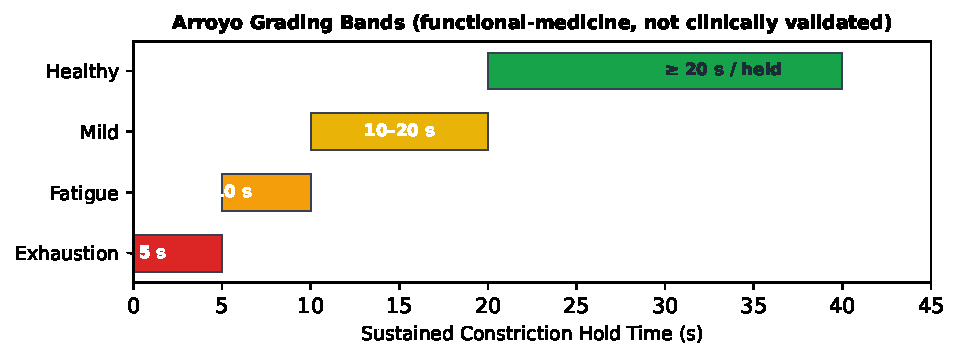
\includegraphics[width=0.95\textwidth]{figures/fig4_grading_bands.pdf}
  \caption{Grading threshold bands. Hold time is mapped to four functional
  bands: healthy ($\geq$\,20\,s), mild (10--20\,s), fatigue (5--10\,s), and
  exhaustion ($<$\,5\,s). These are screening bands, not validated
  diagnostic thresholds.}
\end{figure}

\begin{figure}[htbp]
  \centering
  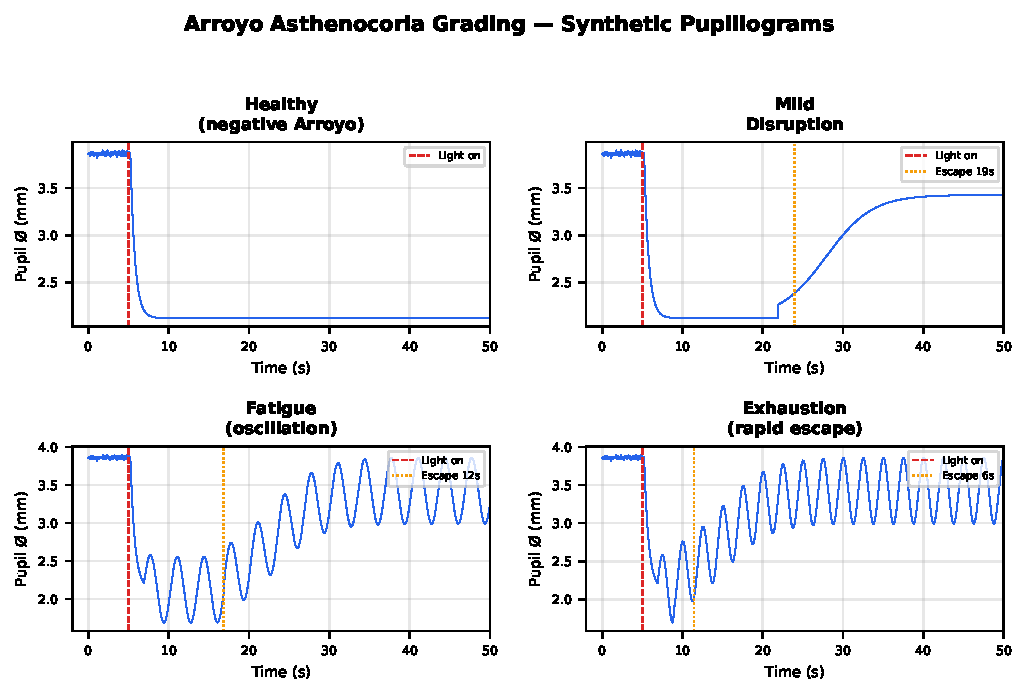
\includegraphics[width=0.90\textwidth]{figures/fig1_grades.pdf}
  \caption{Four-grade pupillogram comparison. Synthetic pupillograms
  illustrate each grade: healthy (sustained constriction), mild (late
  escape), fatigue (early escape with oscillation), and exhaustion (rapid
  failure).}
\end{figure}

\section{Validation}

The analysis core is validated by a suite of 25 unit tests
(\texttt{tests/test\_analysis.py}) using synthetic pupillograms with known
ground truth. The synthetic generator (\texttt{synth\_eye}) produces
deterministic pupillograms parameterized by escape hold time, oscillation
frequency, constriction fraction, and noise level, allowing each grading
band and edge case to be tested independently.

The test suite covers:

\begin{itemize}
  \item \textbf{Synthetic generator verification} (3 tests): Valid generation
        of healthy and fatigue patterns; blink frame invalidation.
  \item \textbf{Healthy pupil} (4 tests): No escape detected; constriction
        percentage in expected range (30--55\%); valid baseline diameter;
        holding index $>$\,0.80.
  \item \textbf{Mild escape} (3 tests): Escape detected; grade assigned as
        ``mild''; escape time within the 12--22\,s band.
  \item \textbf{Fatigue with oscillation} (3 tests): Escape detected; grade
        ``fatigue''; oscillation count $>$\,5 and frequency $>$\,0.1\,Hz.
  \item \textbf{Exhaustion} (3 tests): Escape detected; grade
        ``exhaustion''; escape time $<$\,8\,s.
  \item \textbf{No reflex} (1 test): Flat pupil (0.1\% constriction) graded
        as ``noReflex''.
  \item \textbf{Insufficient data} (3 tests): Empty sample list; too few
        samples ($<$\,5); majority-invalid frames ($<$\,50\% valid) all
        graded as ``insufficientData''.
  \item \textbf{Session symmetry} (3 tests): Both eyes healthy $\rightarrow$
        overall healthy; disagreeing eyes $\rightarrow$ overall takes worse
        grade; both fatigue $\rightarrow$ overall fatigue.
  \item \textbf{Quality warnings} (2 tests): Low sample rate ($<$\,15\,fps)
        triggers warning; short recording ($<$\,30\,s) triggers warning.
\end{itemize}

All 25 tests pass. The tests are run with Python's \texttt{unittest} framework
and require no external hardware, making them suitable for continuous
integration. The synthetic generator's deterministic seeding (random seed
parameter) ensures reproducibility across test runs.

\section{Discussion}

\subsection{What This System Enables}

For naturopathic and functional medicine practitioners, the \texttt{arroyo-pi}
system transforms Arroyo's test from a subjective observation into a
quantitative measurement. The key benefits are:

\begin{itemize}
  \item \textbf{Objective trend tracking:} A practitioner can record a
        pupillogram at each visit and compare hold times, constriction
        amplitudes, and oscillation patterns over months or years. Changes
        are quantified in seconds and percentages, not described as
        ``better'' or ``worse.''
  \item \textbf{Repeatability:} The 940\,nm IR illumination is invisible to
        the patient, eliminating the confound of the measurement light
        itself affecting the pupil. The PIR calibration method is robust to
        small changes in camera positioning between sessions.
  \item \textbf{Removal of observer bias:} The algorithm applies identical
        criteria to every recording. Two practitioners analyzing the same
        pupillogram will get the same grade, because the grading is
        deterministic.
  \item \textbf{Documentation:} Each exam produces a CSV of the raw
        pupillogram and a JSON report with all metrics, creating a
        longitudinal record that can be reviewed, shared, or audited.
\end{itemize}

\subsection{Comparison to the Apple Vision Pro Approach}

The \texttt{arroyo-pi} system is the hardware successor to
\texttt{arroyo-visionos}, an Apple Vision Pro application that implemented
the same analysis algorithm using the headset's built-in eye-tracking
cameras. The Vision Pro approach had significant advantages: high-quality
eye tracking, controlled IR illumination, and a self-contained headset form
factor. However, Apple's enterprise camera restrictions and the \$3,49
device cost made it impractical for clinical deployment~[12].

The Raspberry Pi / Jetson approach sacrifices some tracking precision but
gains accessibility. A practitioner can assemble the system for under \$100
using off-the-shelf components. The analysis algorithm is identical between
the two platforms---only the data acquisition layer differs.

\subsection{Comparison to Research-Grade Pupillometers}

OpenIris is an open-source eye-tracking framework that achieves 500\,Hz
sampling with FLIR machine-vision cameras, providing millisecond-resolution
pupillary dynamics~[15,21]. The MEYELens system is an open-source
pupil\-lom\-etry eyewear platform for mobile measurement~[20].
Smart\-phone-based pupillometry approaches have also been validated
against clinical instruments~[11,12].

The \texttt{arroyo-pi} system operates at 30\,fps with consumer cameras, two
orders of magnitude slower than OpenIris. However, the Arroyo test operates
on a timescale of seconds, not milliseconds. The critical measurements are
hold time (seconds), escape threshold crossing (sustained over 2\,s), and
oscillation frequency ($\sim$0.3\,Hz). A 30\,fps sampling rate provides
33\,ms temporal resolution, which is more than adequate for these dynamics.
The trade-off is clear: the system exchanges high-speed precision for
low-cost accessibility, and for the Arroyo test specifically, this is a
reasonable exchange.

Raspberry Pi-based ophthalmic imaging has precedent: Shen and Mukai
demonstrated a Pi-based fundus camera~[14], and the Raspberry Pi Foundation
has highlighted affordable ocular imaging as an application
area~[13]. The \texttt{arroyo-pi} system extends this tradition to
pupillography.

\section{Conclusion}

Arroyo's asthenocoria sign has endured for a century as a clinical
observation without instrumentation. The \texttt{arroyo-pi} system replaces
the penlight-and-stopwatch exam with an embedded pupillography platform that
quantifies pupillary behavior under sustained light using near-infrared
illumination, OpenCV-based tracking, and a deterministic analysis pipeline.

The system is deliberately honest about its limitations. It measures pupillary
behavior, not adrenal function. Its grading thresholds are functional-medicine
screening bands, not validated diagnostic criteria. ``Adrenal fatigue'' is not
a recognized endocrinological diagnosis, and the ACTH stimulation test remains
the gold standard for adrenal insufficiency. Asthenocoria is nonspecific.

What the system provides is objectivity where there was subjectivity,
repeatability where there was inconsistency, and a quantitative record where
there was clinical impression. For practitioners who use Arroyo's test as a
screening and trend-tracking instrument, this is a meaningful improvement.
The sub-\$100 hardware cost and open-source software make it accessible to
the clinics and practices where the test is actually performed.

Future work should focus on clinical validation: comparing the system's
measurements against established pupillometry protocols, characterizing
inter-session variability, and evaluating whether the grading bands
correlate with any validated physiological markers. Until such validation
exists, the system should be used as what it is---a screening instrument that
quantifies an observation, not a diagnostic tool that identifies a disease.

\begin{thebibliography}{99}
\begingroup\sloppy

\bibitem{tpauk} Thyroid Patient Advocacy UK. Tests for adrenal fatigue you can
  do at home. Available at:
  \url{https://www.tpauk.com/main/article/tests-for-adrenal-fatigue-you-can-do-at-home/}

\bibitem{jockers} Dr.\ Jockers. How to test adrenal function: the iris
  contraction test and grading protocol. Available at:
  \url{https://drjockers.com/test-adrenal-function/}

\bibitem{farlex} Farlex Medical Dictionary. Asthenocoria / Arroyo sign.
  Available at:
  \url{https://medical-dictionary.thefreedictionary.com/asthenocoria}

\bibitem{iqb} IQB Spanish Medical Dictionary. Signo de ARROYO. Available at:
  \url{https://www.iqb.es/diccio/s/signo.htm}

\bibitem{garma} Garma on Health. Adrenal fatigue tests you can do: the
  8-inch, 45-degree protocol. Available at:
  \url{https://garmaonhealth.com/adrenal-fatigue-tests-you-can-do/}

\bibitem{pulaski} Pulaski, S. Alpha Omega Pupil: syntonic optometry and
  pupillary response. Syntonic Academy. Available at:
  \url{https://csovision.org/wp-content/uploads/2020/05/Syntonic2020AOPupilShort101ZoomAlbanyPDFX.pdf}

\bibitem{szabadi} Szabadi, E. (2018). Regulation of the pupil by the
  sympathetic pathways. \textit{Journal of Neurology, Neurosurgery \&
  Psychiatry}, PMC6305320. Available at:
  \url{https://pmc.ncbi.nlm.nih.gov/articles/PMC6305320/}

\bibitem{hall} Hall, C.A.\ \& Chilcott, R.P.\ (2018). Pupillary light reflex
  in neurodiagnostics. PMC5872002. Available at:
  \url{https://pmc.ncbi.nlm.nih.gov/articles/PMC5872002/}

\bibitem{ulyclinic} Ulyclinic. Asthenocoria (Arroyo's sign). Available at:
  \url{https://www.ulyclinic.com/cardiovascular-disease-conditions/asthenocoria-(arroyo's-sign)}

\bibitem{amboss} AMBOSS. Adrenal insufficiency: ACTH stimulation test.
  Available at: \url{https://www.amboss.com/us/knowledge/adrenal-insufficiency}

\bibitem{kuthe} Kuthe, S.\ \& Lakhe, S.\ (2025). Smartphone pupillometry:
  methods and validation. PMC12391761. Available at:
  \url{https://pmc.ncbi.nlm.nih.gov/articles/PMC12391761/}

\bibitem{homepupil} At-home pupillometry: smartphone validation against
  clinical instruments. PMC10686294. Available at:
  \url{https://pmc.ncbi.nlm.nih.gov/articles/PMC10686294/}

\bibitem{rpfundus} Raspberry Pi Foundation. An affordable ocular fundus
  camera. Available at:
  \url{https://www.raspberrypi.com/news/an-affordable-ocular-fundus-camera/}

\bibitem{shen} Shen, A.\ \& Mukai, S.\ (2017). A low-cost Raspberry
  Pi-based fundus camera. PMC5370517. Available at:
  \url{https://pmc.ncbi.nlm.nih.gov/articles/PMC5370517/}

\bibitem{openirisdpi} OpenIrisDPI: an open-source eye tracking and
  pupillometry framework. PMC12900282. Available at:
  \url{https://pmc.ncbi.nlm.nih.gov/articles/PMC12900282/}

\bibitem{dsouza} Dsouza, J. InfraredPupilTracker: pupil tracking on
  Raspberry Pi with OpenCV. GitHub repository. Available at:
  \url{https://github.com/JohnalDsouza/InfraredPupilTracker}

\bibitem{arducam} Arducam. IMX462 Pivariety camera documentation. Available
  at: \url{https://docs.arducam.com/Raspberry-Pi-Camera/Pivariety-Camera/IMX462/}

\bibitem{amsosram} ams OSRAM. 940\,nm IR for eye, face, and hand tracking.
  Available at:
  \url{https://ams-osram.com/applications/mobile-wearables/eye-face-hand-tracking}

\bibitem{babcock} Babcock, J.S.\ \& Pelz, J.B.\ (2004). Building a
  lightweight eyetracking headgear. \textit{ETRA 2004}. Available at:
  \url{https://www.cis.rit.edu/people/faculty/pelz/publications/ETRA04_babcock_pelzOLD.pdf}

\bibitem{meyelens} Vecchieschi, P.\ et al.\ (2026). MEYELens: open-source
  pupillometry eyewear. \textit{Behavior Research Methods}. Available at:
  \url{https://ricerca.sns.it/retrieve/359895a9-ea53-4b65-8713-e75673bef581/Vecchieschi_et_al-2026-Behavior_Research_Methods.pdf}

\bibitem{openiris} OpenIris: an open-source framework for eye tracking.
  ACM Digital Library. Available at:
  \url{https://dl.acm.org/doi/pdf/10.1145/3649902.3653348}

\bibitem{pinn} Pinn Clinic. Adrenal fatigue and Wilson's 1998 framework.
  Available at: \url{https://www.pinnclinic.com/adrenal-fatigue}

\bibitem{adrenalfatigue} Adrenal Fatigue Solution. Testing for adrenal
  fatigue: the iris contraction test. Available at:
  \url{https://adrenalfatiguesolution.com/testing-for-adrenal-fatigue/}

\bibitem{clinicalgate} Clinical Gate. Naturopathic diagnostic techniques.
  Available at: \url{https://clinicalgate.com/2015/05/27/naturopathic-diagnostic-techniques/}

\bibitem{darwyn} Darwyn Health. Naturopathic diagnostic methods: a
  comprehensive guide. Available at:
  \href{https://www.darwynhealth.com/alternative-medicine/naturopathy/principles-of-naturopathy/naturopathic-diagnostic-methods/a-comprehensive-guide-to-naturopathic-diagnostic-methods-for-improved-wellness/}{darwynhealth.com}

\bibitem{kelbsch} Kelbsch, C.\ et al.\ (2023). Pupillary escape and the
  Loewenfeld legacy. PMC10199107. Available at:
  \url{https://pmc.ncbi.nlm.nih.gov/articles/PMC10199107/}

\bibitem{mathot} Math\^ot, S.\ (2018). Pupillometry: a review of methods
  and applications. \textit{Journal of Cognition}. Available at:
  \url{https://journalofcognition.org/articles/10.5334/joc.18}

\bibitem{browning} Browning, M.\ et al.\ Pupillary measures: guidelines
  for researchers. \textit{Psychophysiology}. Available at:
  \url{https://onlinelibrary.wiley.com/doi/10.1111/psyp.14035}

\bibitem{webmd} WebMD. Adrenal fatigue: is it real? Available at:
  \url{https://www.webmd.com/a-to-z-guides/adrenal-fatigue-is-it-real}

\bibitem{clineduc} Clinical Education. Adrenal fatigue, adrenal
  insufficiency, or a misnamed state of hypofunction. Available at:
  \url{https://www.clinicaleducation.org/resources/reviews/adrenal-fatigue-adrenal-insufficiency-or-a-misnamed-state-of-hypofunction/}

\bibitem{mnt} Medical News Today. Adrenal fatigue myths. Available at:
  \url{https://www.medicalnewstoday.com/articles/245810}

\end{thebibliography}
\endgroup

\end{document}